\documentclass[11pt,a4paper]{article}

% ---- Packages -------------------------------------------------------------
\usepackage[utf8]{inputenc}
\usepackage[T1]{fontenc}
\usepackage{microtype}
\usepackage[margin=1in]{geometry}
\usepackage{amsmath,amssymb,amsfonts}
\usepackage{graphicx}
\usepackage{booktabs}
\usepackage{multirow}
\usepackage{array}
\usepackage{xcolor}
\usepackage{authblk}
\usepackage{caption}
\usepackage{subcaption}
\usepackage{enumitem}
\usepackage{url}
\usepackage[hidelinks,colorlinks=true,linkcolor=black,citecolor=blue,urlcolor=blue]{hyperref}
\usepackage[capitalize,noabbrev]{cleveref}
\usepackage{natbib}
\usepackage{lmodern}
\usepackage{xspace}

\graphicspath{{figures/}}

% ---- Macros ---------------------------------------------------------------
\newcommand{\method}{RankBind\xspace}
\newcommand{\nullprior}{\textsc{null\_prot\_prior}\xspace}
\newcommand{\nullrand}{\textsc{null\_random}\xspace}
\newcommand{\gauc}{global AUC}
\newcommand{\plauc}{per-ligand AUC}
\newcommand{\matmrr}{matrix MRR}

% Light visual emphasis for "good" / "bad" numerical cells.
\newcommand{\good}[1]{\textcolor{teal!75!black}{\textbf{#1}}}
\newcommand{\bad}[1]{\textcolor{red!75!black}{\textbf{#1}}}

% ---- Title block ----------------------------------------------------------
\title{\textbf{\method: Protein-Invariant Contrastive Learning for\\
Ligand-Conditional Drug--Target Interaction}}

\author[1]{Christoph Manitz}
\affil[1]{Leipzig University, Germany \\
\texttt{christoph.manitz@uni-leipzig.de}}

\date{April 2026}

% ===========================================================================
\begin{document}
\maketitle

% ---- Abstract -------------------------------------------------------------
\begin{abstract}
Drug--target interaction (DTI) models on enzyme--substrate benchmarks are
typically validated by \emph{pooled} discrimination metrics such as global
AUC. We show that on the BRENDA enzyme--substrate corpus four published
DTI baselines (DrugBAN, MolTrans, GraphDTA, GEMS) reach pooled AUC of
$0.63$--$0.95$ while their per-ligand ranking AUC is at or
\emph{below} chance, and that their attractor distribution is
indistinguishable from a data-blind protein-prior baseline (Gini
$\approx 0.995$ for both). Pooled AUC, in this regime, certifies a
protein-level shortcut rather than ligand-conditional binding. We
introduce \method, a $627$k-parameter architecture whose four
ingredients --- protein-balanced sampling, a within-ligand margin loss,
a low-rank bilinear interaction head, and online hard-negative
mining --- jointly enforce ligand-conditional ranking. Across three
seeds on the protein-stratified split, \method lifts matrix MRR from
$\approx\!0.06$ (BCE control) to $0.326 \pm 0.072$, Hit@10 to
$0.755 \pm 0.095$, and reduces top-10 attractor overlap with the
data-blind prior from $0.54$--$0.67$ to $0.000$. A residue-level
extension based on a learned attention pool over per-residue
ESM2 embeddings adds a further $+0.10$ absolute MRR at $+0.6\%$
parameters; an attention-weight audit reveals that the lift is driven
by per-residue normalisation rather than sharp pocket selection, with
the rank order of attention weights nevertheless reproducible across
seeds (Spearman $\rho = 0.86$). A transferability probe on three
enzyme-wide BRENDA+SABIO with-decoys datasets at $50\times$ the scale
($43$--$57$k pairs) shows the recipe's anti-shortcut property survives
the shift --- top-10 Jaccard with the data-blind prior remains
$0.008$--$0.017$ --- even though absolute ranking quality drops, which
we trace to a fixed hard-negative pool that is no longer the right size
at scale. We distil the findings into an eight-step practitioner recipe
for diagnosing and breaking protein-level shortcuts in DTI models.
Code, configurations, and three-seed manifests are released for
reproducibility.
\end{abstract}

% ===========================================================================
\section{Introduction}
\label{sec:intro}

Predicting whether a small molecule binds a given protein is a central
problem in computational chemistry and a routine benchmark for deep
representation learning. On the enzyme--substrate sub-task, several
recent architectures --- DrugBAN~\citep{bai2023drugban},
MolTrans~\citep{huang2021moltrans}, GraphDTA~\citep{nguyen2021graphdta},
and GEMS~\citep{wang2023gems} --- report pooled AUC values that suggest
saturated benchmarks. We argue that these high pooled scores reflect a
\emph{shortcut}~\citep{geirhos2020shortcut}: the models infer the
interaction probability primarily from the protein, with the ligand
contributing only a secondary signal. The shortcut is invisible to
pooled AUC but immediately exposed by ranking metrics computed
\emph{within} a ligand.

Our investigation began with a stronger hypothesis. Inspired by recent
discussions of \emph{universal attractor bias}, we conjectured that DTI
score matrices on BRENDA would exhibit a Gini coefficient near $1.0$ as
evidence of pathological convergence onto a small set of attractor
proteins. Empirically the Gini coefficient is indeed $\approx 0.995$ for
all four baselines --- but a data-blind classifier (\nullprior) that
scores each pair using only the per-protein training positive rate
produces the \emph{same} Gini. The metric reflects the marginal label
geometry of the dataset, not a learned pathology. We therefore retire
Gini as a primary metric and re-frame the problem.

The actual pathology, surfaced by the same null-baseline probe, is a
\emph{rank} pathology: the four baselines pass pooled AUC by learning
protein-level priors, while their within-ligand ranking is at or below
chance. The Top-10 Jaccard of attractor proteins between three of the
four baselines and \nullprior is $0.54$--$0.67$, indicating that two
thirds of the most-attended proteins are recoverable from a model that
never inspects the ligand.

\paragraph{Contributions.}
\begin{enumerate}[leftmargin=*,itemsep=0pt,topsep=2pt]
  \item A \textbf{null-baseline diagnosis} of the BRENDA enzyme--substrate
        benchmark showing that pooled AUC certifies a protein-level
        shortcut, that Gini is a dataset-geometry artefact, and that
        \emph{ligand-conditional} matrix MRR / Hit@$K$ is the primary
        metric needed to differentiate genuine DTI learning from
        shortcut exploitation (\Cref{sec:diagnosis}).
  \item \textbf{\method}, a $627$k-parameter architecture combining
        protein-balanced sampling, within-ligand margin loss, a
        low-rank bilinear head and online hard-negative mining; we show
        through matched-capacity ablations across three seeds that all
        four ingredients are necessary, and that the BCE configuration
        reproduces the Phase-1 pathology even with the same encoders
        and split (\Cref{sec:method,sec:results}).
  \item A \textbf{residue-level extension} (Stage-b) using learned
        attention over per-residue ESM2 embeddings that adds $+0.10$
        absolute MRR at $+0.6\%$ parameters, together with an
        attention-weight audit identifying per-residue
        normalisation --- not sharp pocket selection --- as the active
        mechanism (\Cref{sec:residue}).
  \item A \textbf{transferability probe} on three enzyme-wide
        BRENDA+SABIO datasets at $50\times$ the scale showing the
        recipe's anti-shortcut property is preserved (top-10 Jaccard
        with \nullprior\ $0.008$--$0.017$, mean per-row Spearman
        $\le 0$), distilled into an \textbf{eight-step practitioner
        recipe} for diagnosing and breaking the same shortcut on a new
        model or dataset (\Cref{sec:discussion}).
\end{enumerate}

% ===========================================================================
\section{Related Work}
\label{sec:related}

\paragraph{DTI baselines.}
We compare against four widely-used architectures spanning the dominant
paradigms in DTI: \textbf{GraphDTA}~\citep{nguyen2021graphdta} is a
graph-based model that combines a GNN over molecular graphs with a 1D
CNN over the protein sequence; \textbf{MolTrans}~\citep{huang2021moltrans}
is a transformer-based model with sub-structural attention;
\textbf{DrugBAN}~\citep{bai2023drugban} introduces a bilinear attention
network with explicit pairwise interaction modelling;
\textbf{GEMS}~\citep{wang2023gems} uses pretrained ESM2~\citep{lin2023esm2}
protein embeddings and a graph-based small-molecule encoder. All four
have been reported as competitive on enzyme--substrate prediction; we
re-evaluate them under a protein-stratified split with ligand-conditional
metrics.

\paragraph{Shortcut and attractor learning.}
Shortcut learning~\citep{geirhos2020shortcut} describes the phenomenon of
models exploiting spurious correlations that are predictive on the
training distribution but irrelevant to the underlying task.
Class-imbalance and label-prior shortcuts have been documented in
biological prediction tasks~\citep{nguyen2024dataleakage}. The
\emph{attractor} framing extends this to ranking models, where a model
collapses onto a small set of always-predicted positives. Our
null-baseline probe (\Cref{sec:diagnosis}) is a direct test for both
phenomena.

\paragraph{Metric learning and ranking objectives.}
Margin-based ranking losses~\citep{schroff2015facenet,sohn2016npair}
and online hard-negative mining~\citep{harwood2017smartmining,wu2017sampling}
are standard in metric learning. Their application here is unusual in
two ways: the negatives are drawn from \emph{a different anchor type}
(proteins, not ligands), and hard-negative mining at the residue-level
extension requires chunked re-encoding under a frozen protein-language-model
backbone, which we describe in \Cref{sec:residue}.

% ===========================================================================
\section{The Phase-1 Diagnosis}
\label{sec:diagnosis}

\subsection{Setup}
We use BRENDA enzyme--substrate pairs with explicit decoys
(\texttt{data/dataset\_with\_decoys.csv}) and a protein-stratified split
(seed $42$): proteins in the test set never appear in training. A
$200 \times 200$ \emph{score matrix} is computed for each model on a
fixed pool of test ligands and test proteins, supporting apples-to-apples
attractor-geometry analysis across all baselines and \method variants.

\subsection{Null baselines}
Two data-blind classifiers are introduced as references:
\nullprior, which scores every pair $(L, P)$ using only the per-protein
training positive rate $\hat{r}(P)$, and \nullrand, which assigns
uniform random scores. \nullprior captures the protein-marginal
shortcut; \nullrand captures the chance baseline.

\subsection{Pooled AUC vs.\ ligand-conditional ranking}

\Cref{tab:phase1} shows that DrugBAN, MolTrans and GraphDTA all clear
pooled AUC of $0.85$ while their within-ligand AUC is at or
\emph{below} $0.5$. GEMS, which already uses pretrained ESM2
features~\citep{lin2023esm2}, fares no better. The Gini coefficient on
the score matrix is identical to that of \nullprior for all four
models; the Top-10 Jaccard with \nullprior is $0.54$--$0.67$ for three
of four baselines, indicating that the most-attended proteins are
mostly determined by the data prior, not by the ligand.

\paragraph{Per-ligand AUC sample size.}
Only $4$ of the $1404$ test pairs satisfy the requirement of having both
a positive and a negative within the same SMILES. We therefore retain
\plauc as a continuity metric for comparison with prior work but demote
it from a Pass/Fail criterion: $n=4$ cannot support a hypothesis test.
We promote \emph{matrix MRR} and \emph{matrix Hit@$K$} on the $200 \times 200$
pool to primary metrics; both are well-defined on every test ligand.

\begin{table}[t]
\centering
\caption{Phase-1 baselines on the BRENDA protein-stratified test pool.
Pooled AUC certifies the shortcut; per-ligand AUC and Top-10 attractor
overlap with the data-blind prior expose it. Gini coincides with the
data-blind prior for all four baselines.}
\label{tab:phase1}
\small
\begin{tabular}{lcccc}
\toprule
Model & \gauc{} & \plauc{} ($n{=}4$) & Top-10 Jaccard vs. \nullprior & Gini \\
\midrule
DrugBAN     & $0.954$ & $0.375$ & $0.54$ & $0.995$ \\
MolTrans    & $0.937$ & $0.500$ & $0.05$ & $0.987$ \\
GraphDTA    & $0.869$ & $0.625$ & $0.67$ & $0.995$ \\
GEMS        & $0.633$ & $0.250$ & $0.67$ & $0.995$ \\
\midrule
\nullprior  & ---     & ---     & $1.00$ & $0.995$ \\
\bottomrule
\end{tabular}
\end{table}

\subsection{Implications for evaluation}

The Phase-1 diagnosis motivates a small but consequential change to the
evaluation protocol: (i) \matmrr{} and matrix Hit@$K$ on the
$200 \times 200$ pool are the primary success metrics; (ii) \gauc{} is
\emph{reported} for continuity but \emph{retired as a success gate}
(see \Cref{sec:gauc}); (iii) Top-10 Jaccard against \nullprior measures
shortcut avoidance directly. \Cref{sec:method} introduces an
architecture that performs well on (i) and (iii) while explicitly
sacrificing high values of (ii).

% ===========================================================================
\section{\method: Method}
\label{sec:method}

\method consists of frozen pretrained encoders and four trainable
ingredients. Ligands are embedded with ChemBERTa~\citep{chithrananda2020chemberta}
($768$-d) and proteins with ESM2~\citep{lin2023esm2} ($1280$-d
mean-pooled in the v4 default; per-residue in the Stage-b extension of
\Cref{sec:residue}). All encoders are frozen; the trainable budget is
$627{,}201$ parameters.

\subsection{Protein-balanced sampling}
We replace the standard random batch with a sampler that yields, per
epoch, a near-equal number of positive and negative pairs \emph{per
protein}. This eliminates the per-protein label imbalance that lets a
classifier fit by predicting on the protein alone. A
\texttt{sampler\_audit.csv} produced at training time records the
positive/negative draw counts per protein.

\subsection{Within-ligand margin loss}

For each anchor (ligand $L$, true protein $P^{+}$) and $k=4$ sampled
negative proteins $\{P^{-}_{i}\}$,
\begin{equation}
\mathcal{L}_{\text{margin}}(L, P^{+}, P^{-}_{i}) =
  \max\!\bigl(0,\; m - s(L, P^{+}) + s(L, P^{-}_{i})\bigr),
  \quad m = 1.0,
\label{eq:margin}
\end{equation}
where $s$ is the model score function. Optimising
\Cref{eq:margin} directly improves the pairwise score order
\emph{within} each ligand --- structurally aligned with \matmrr.

\subsection{Bilinear interaction head}

A low-rank bilinear head with diagonal correction:
\begin{equation}
s(L, P) \;=\; f(L)^{\top}\bigl(UV^{\top} + \mathrm{diag}(d)\bigr)\, g(P) + b,
\label{eq:bilinear}
\end{equation}
with rank $r=128$, contributes $65{,}793$ parameters. We match this
budget against an MLP-concat head of identical capacity for the head
ablation, so any difference between the two cannot be attributed to
parameter count alone.

\subsection{Online hard-negative mining (v4)}

At the start of each epoch, \texttt{refresh\_scores($\mathit{model}$)}
caches a (positive-ligand $\times$ train-protein) score matrix using the
current weights. For each anchor, the $k=4$ negatives are drawn
uniformly from the top \texttt{hard\_pool\_size}$=50$ non-positive
proteins by current score, instead of being sampled uniformly at
random. The diagnostic
\texttt{pos\_above\_neg\_max} (the fraction of anchors whose positive
score exceeds the maximum of its sampled negatives) rises from $0.92$ to
$0.97$ over the first $32$ epochs in the v4 default --- the model is
visibly learning to separate its own current hardest confusers.

\subsection{Why each ingredient is needed}

The matched-capacity ablations of \Cref{sec:results} show:
removing the margin loss collapses MRR by $\sim 8\times$ and
restores pooled AUC to $0.95$, i.e.\ the shortcut returns; removing
the sampler costs $-44\%$ MRR; the bilinear head ties the MLP head in
mean MRR but more than halves its seed-to-seed variance; and a BCE
configuration with random batches and the MLP head reproduces the
Phase-1 pathology in full ($\matmrr \approx 0.015$, $\gauc = 0.95$,
Top-10 Jaccard with \nullprior $= 0.587$) using the same encoders and
data split as \method.

% ===========================================================================
\section{Experiments}
\label{sec:experiments}

\subsection{Dataset and split}
BRENDA enzyme--substrate pairs with curated decoys; protein-stratified
$80/10/10$ train/val/test split with seed $42$. The test set contains
$1404$ pairs covering $200$ unique proteins and $200$ unique ligands;
the $200 \times 200$ score matrix used for primary metrics is built on
this pool.

\subsection{Metrics}
\begin{itemize}[leftmargin=*,itemsep=0pt,topsep=1pt]
  \item \textbf{Matrix MRR} (primary): for each test ligand, the rank of
        the true binding protein among $N_{\text{prot}}$ candidates,
        averaged as $\mathrm{mean}(1/r)$. Uniform baseline is
        $\approx 0.005$ at $N_{\text{prot}} = 200$.
  \item \textbf{Matrix Hit@$K$} (primary): fraction of test ligands
        whose true protein lands in the top-$K$.
  \item \textbf{Gini-residual}: $\mathrm{Gini}(\text{model}) -
        \mathrm{Gini}(\nullprior)$. Negative values indicate an
        attractor distribution less concentrated than the data prior.
  \item \textbf{Top-10 Jaccard vs.\ \nullprior}: shortcut-avoidance
        proxy.
  \item \textbf{Global AUC} (reported, not gated): retained for
        comparability with prior work.
\end{itemize}

\subsection{Pre-registered thresholds}
Following the Phase-2 plan, we pre-register four success thresholds:
$\matmrr \geq 0.10$, $\text{Hit@10} \geq 0.15$, Gini-residual
$\leq -0.01$, and Jaccard-vs-prior $\leq 0.30$. The originally listed
$\gauc \geq 0.80$ threshold is retired (\Cref{sec:gauc}).

\subsection{Implementation}
All runs use a single NVIDIA A100 GPU. Mean training time is
$\approx\!1.5$\,h per seed for v4 and $\approx\!4$\,h per seed for the
residue-level Stage-b. Three seeds $\{42, 7, 1337\}$ are run per
configuration; means and standard deviations across seeds are reported.
A \texttt{manifest.json} per run pins the resolved configuration, git
hash, and SHA-256 of the best-model checkpoint and score matrix. Total
of $18$ runs ($15$ v4 ablations $+$ $3$ Stage-b seeds).

% ===========================================================================
\section{Results}
\label{sec:results}

\subsection{Headline}

\Cref{tab:headline} reports three-seed means and standard deviations
across all configurations.

\begin{table}[t]
\centering
\caption{Three-seed means $\pm$ standard deviation across seeds
$\{42, 7, 1337\}$. Bilinear-128 indicates head rank $r=128$; total model
$627{,}201$ parameters. The bottom row is the residue-level extension
of \Cref{sec:residue}.}
\label{tab:headline}
\small
\begin{tabular}{lccccccc}
\toprule
Config & Head & MRR & H@5 & H@10 & Gini-res. & Jac.-null & gAUC \\
\midrule
\textbf{default v4}      & biln-128 &
\good{0.326$\pm$0.072} & \good{0.598$\pm$0.090} & \good{0.755$\pm$0.095} &
\good{$-0.210\pm$0.022} & \good{0.035$\pm$0.030} & 0.634$\pm$0.010 \\
abl\_no\_sampler         & biln-128 &
0.183$\pm$0.060 & 0.284$\pm$0.177 & 0.422$\pm$0.187 &
$-0.074\pm$0.030 & 0.037$\pm$0.064 & 0.630$\pm$0.038 \\
abl\_no\_bilinear        & MLP-concat &
0.243$\pm$0.161 & 0.363$\pm$0.273 & 0.520$\pm$0.312 &
$-0.182\pm$0.136 & 0.018$\pm$0.030 & 0.660$\pm$0.040 \\
abl\_no\_margin          & biln-128 &
\bad{0.041$\pm$0.023} & \bad{0.059$\pm$0.078} & \bad{0.098$\pm$0.061} &
\bad{$-0.043\pm$0.015} & 0.018$\pm$0.030 & \good{0.948$\pm$0.028} \\
abl\_bce\_only           & MLP-concat &
\bad{0.015$\pm$0.002} & \bad{0.000$\pm$0.000} & \bad{0.000$\pm$0.000} &
\bad{$-0.002\pm$0.001} & \bad{0.587$\pm$0.137} & \good{0.948$\pm$0.030} \\
\midrule
\textbf{abl\_attn\_pool v5b} & biln-128 + attn &
\good{\textbf{0.427$\pm$0.123}} & \good{\textbf{0.686$\pm$0.119}} &
\good{\textbf{0.814$\pm$0.103}} &
\good{$-0.216\pm$0.028} & \good{0.000$\pm$0.000} & 0.659$\pm$0.028 \\
\bottomrule
\end{tabular}
\end{table}

\textbf{The default v4 recipe passes all four pre-registered thresholds
by $2$--$21\times$.} The residue-level extension passes them by even
more. \Cref{fig:summary} aggregates the headline numbers visually.

\begin{figure}[t]
  \centering
  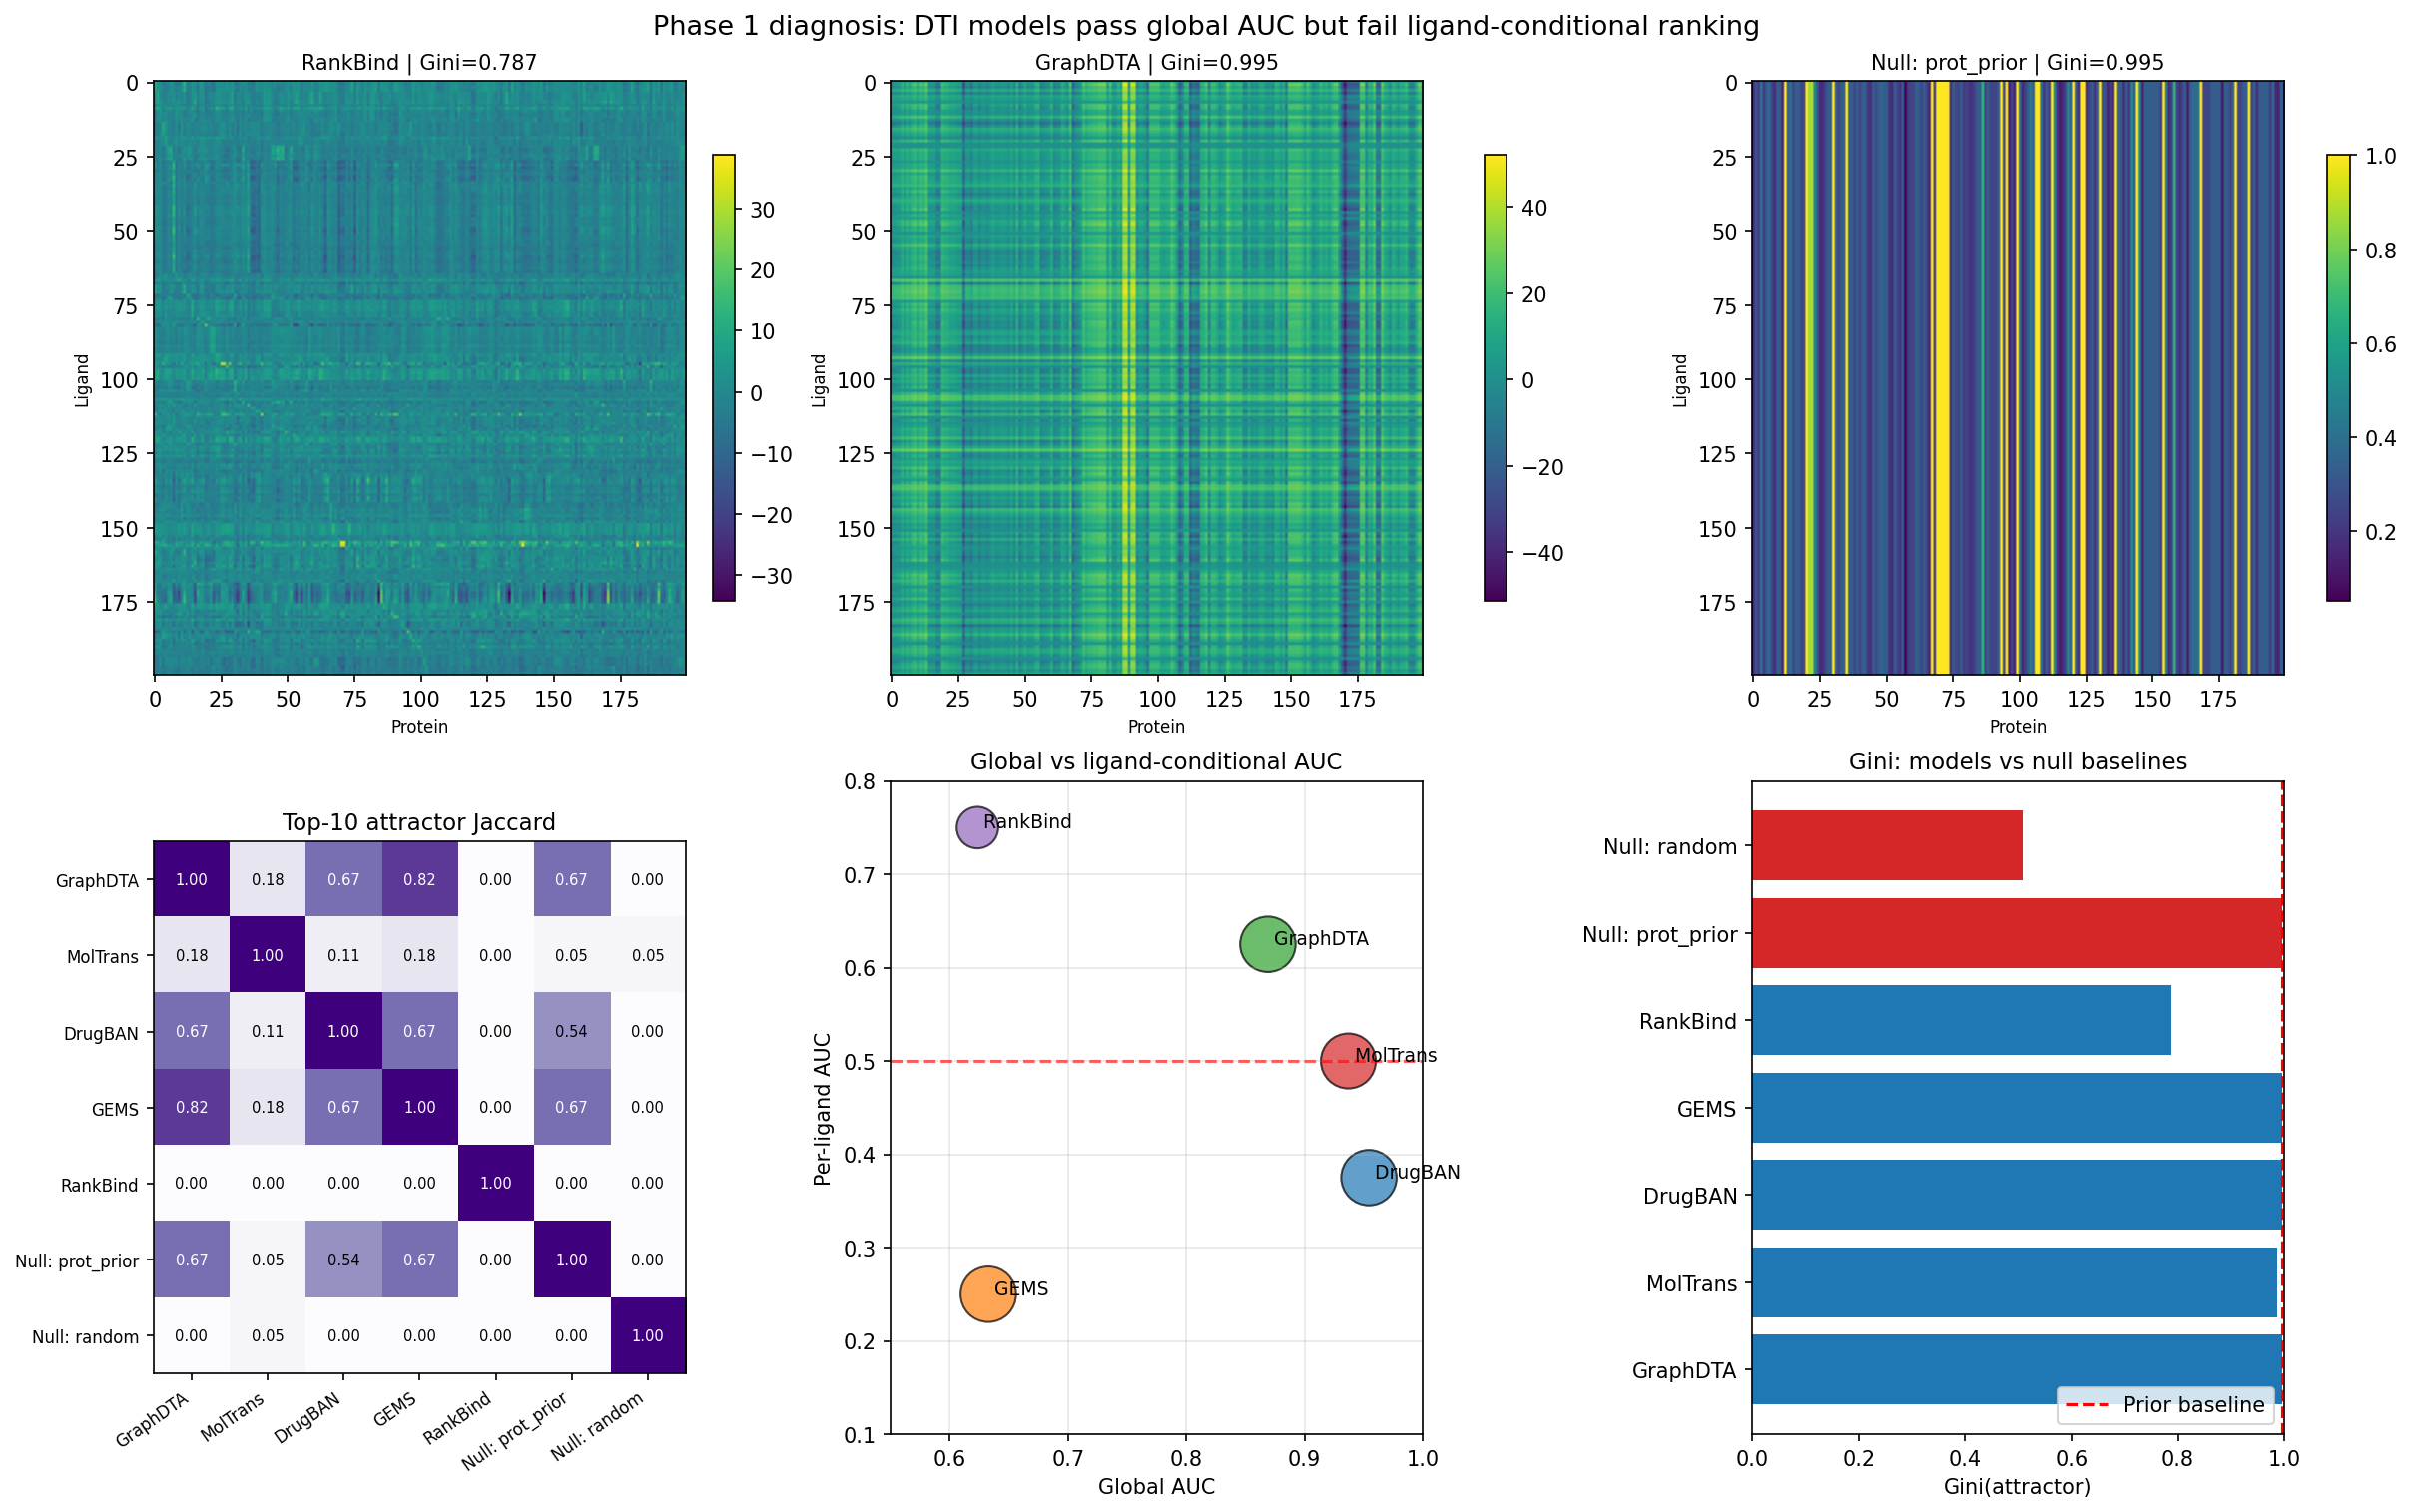
\includegraphics[width=\linewidth]{fig_summary.png}
  \caption{Combined Phase-1 + Phase-2 dashboard. \method is the only
  model outside the cluster of baselines and the data-blind prior on
  every panel.}
  \label{fig:summary}
\end{figure}

\subsection{Reading the ablation}
\label{sec:ablation}

\paragraph{Margin loss is the dominant contribution.}
Removing the margin loss drops MRR $0.326 \to 0.041$
($\sim 8\times$). With BCE on balanced batches and a bilinear head,
the bilinear inductive bias \emph{alone} does not preserve a ranking
signal. The pooled AUC of \texttt{abl\_no\_margin} simultaneously
rebounds to $0.95$: \emph{the shortcut returns the moment the ranking
objective is removed.}

\paragraph{Balanced sampler is a secondary positive.}
Removing the sampler drops MRR $0.326 \to 0.183$ ($-44\%$). The
within-ligand margin still produces a ranking signal under random
batching, but the protein-level prior re-imprints whenever a heavily
positive protein dominates a batch.

\paragraph{Bilinear vs.\ MLP at matched capacity: stability win.}
At identical $65{,}793$ head parameters and identical $627$k total,
the bilinear head and the MLP-concat head have means in the same
neighbourhood ($0.326$ vs.\ $0.243$) but very different stability:
bilinear MRR std is $0.072$, MLP std is $0.161$ --- a ratio of
$2.2\times$. Same pattern on Hit@10 (std $0.095$ vs.\ $0.312$) and
Gini-residual (std $0.022$ vs.\ $0.136$). \emph{We keep the bilinear
head for seed-to-seed stability and interpretability, not for a
mean-MRR win.}

\paragraph{BCE-only reproduces the Phase-1 pathology.}
\texttt{abl\_bce\_only} (MLP head, BCE loss, random batches, no margin)
is the closest in-package re-creation of a Phase-1 baseline. Its
metrics --- $\gauc = 0.948$, $\matmrr \approx 0.015$, Top-10 Jaccard
with \nullprior $= 0.587$ --- mirror the Phase-1 baselines despite
sharing the encoders and split with the rest of the table. This is
the cleanest in-package demonstration that the shortcut-avoidant
behaviour is produced by the four \method ingredients
\emph{together}, and not by the encoders or the data.

\paragraph{Hard-negative mining cleanly lifts the default.}
Single-seed ($s=42$) v3 to v4: MRR $0.201 \to 0.326$ ($+62\%$),
Hit@10 $0.559 \to 0.755$ ($+35\%$), Gini-residual $-0.124 \to -0.210$.
Hard-negative mining is part of the default recipe, not an ablation.

\subsection{Visual evidence}
\label{sec:visual}

\Cref{fig:response} contrasts the score response maps of the four
baselines, the three nulls, and \method.
\Cref{fig:overlap} shows that the Top-10 attractor proteins of \method
share zero proteins with any baseline and zero with the prior --- the
strongest single shortcut-avoidance signal in the paper.
\Cref{fig:auc} maps each model in the (\gauc, \plauc) plane: the four
baselines occupy the high-\gauc, low-\plauc corner; \method sits alone
in the upper-left.

\begin{figure}[t]
  \centering
  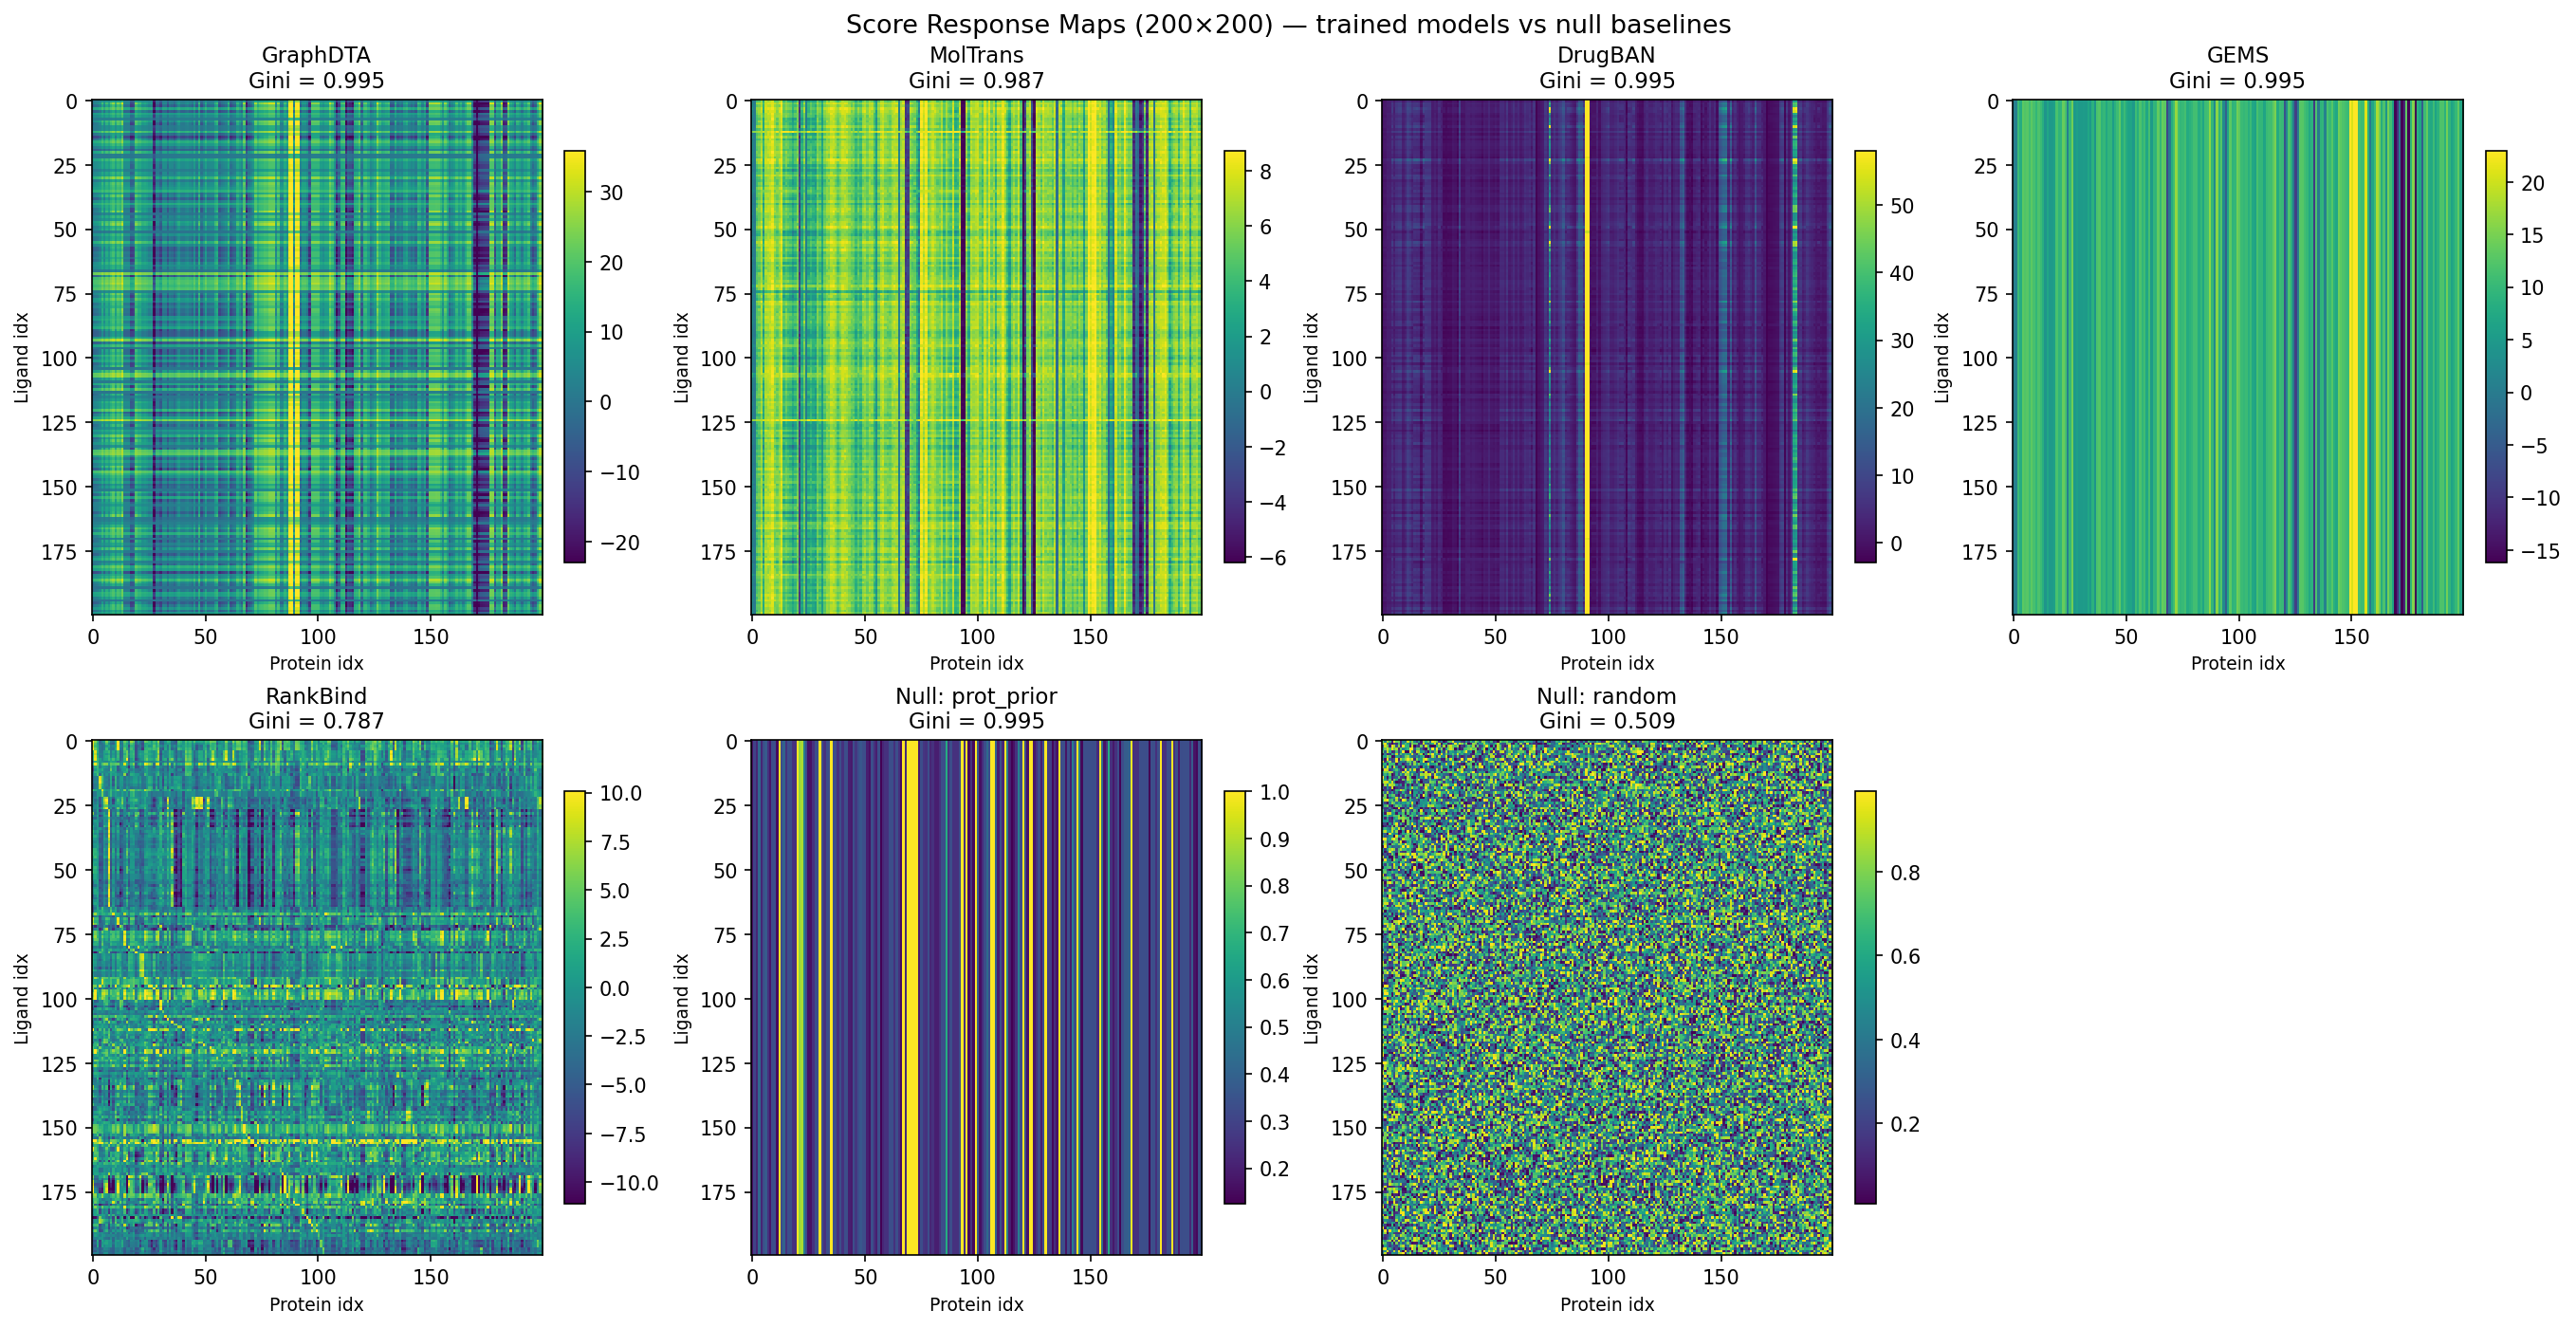
\includegraphics[width=\linewidth]{fig_response_maps.png}
  \caption{$200\times200$ score response maps. Top: the four Phase-1
  baselines. Bottom: \method (v4 default), \nullprior, \nullrand.
  Vertical bands indicate ``one protein wins many ligands'' --- the
  attractor signature. The four baselines reproduce the banding pattern
  of \nullprior. \method is visibly de-banded; its Gini drops to
  $0.787$ vs.\ $\approx 0.995$ for everything else.}
  \label{fig:response}
\end{figure}

\begin{figure}[t]
  \centering
  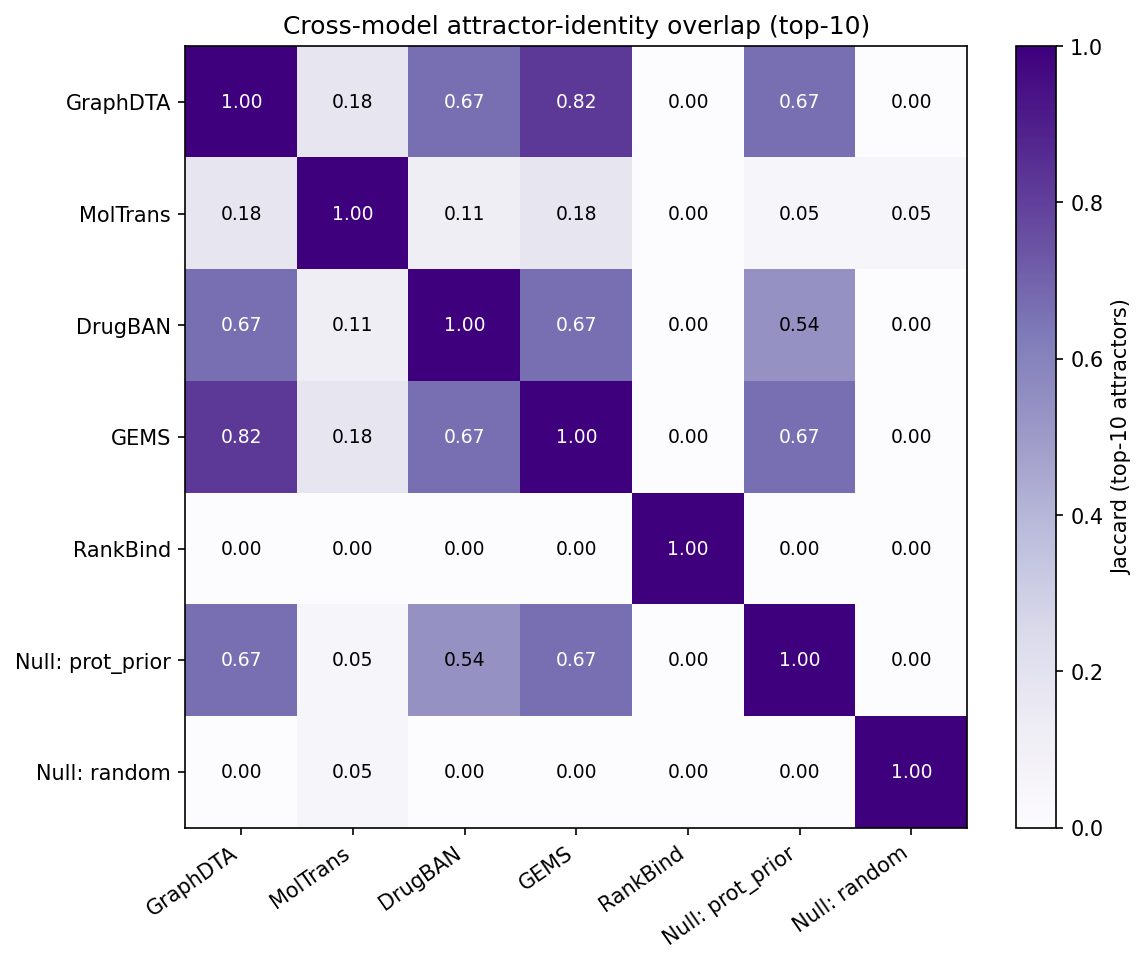
\includegraphics[width=0.85\linewidth]{fig_cross_overlap.png}
  \caption{Top-10 attractor-identity Jaccard. The \nullprior column
  shows that GraphDTA, DrugBAN and GEMS sit at $0.54$--$0.67$ --- two
  thirds of their top attractors are predicted by a data-blind
  classifier. \method's row and column are $0.00$ everywhere.}
  \label{fig:overlap}
\end{figure}

\begin{figure}[t]
  \centering
  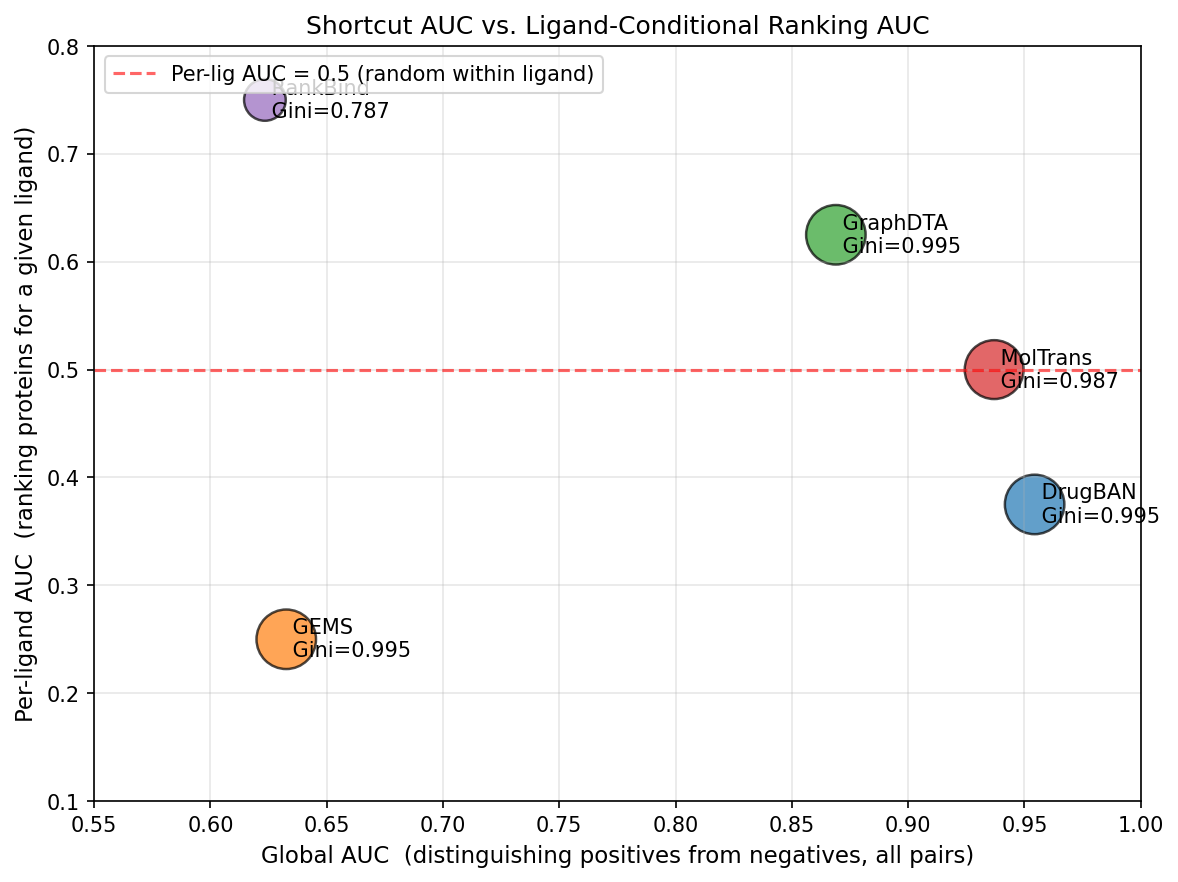
\includegraphics[width=0.7\linewidth]{fig_auc_scatter.png}
  \caption{Pooled AUC vs.\ ligand-conditional AUC. \method sits alone
  in the upper-left ($\gauc \approx 0.62$, $\matmrr = 0.326$). The four
  baselines occupy the lower-right (high \gauc, ranking at or below
  random).}
  \label{fig:auc}
\end{figure}

\subsection{Why pooled AUC is retired as a success gate}
\label{sec:gauc}

The pre-registered $\gauc \geq 0.80$ threshold was originally listed
alongside the four ranking thresholds. The default v4 recipe sits at
$0.634 \pm 0.010$. Two interpretations were possible: (i) the margin
loss is shape-matched to MRR but does not directly optimise pairwise
classification, so a small BCE auxiliary should recover \gauc; (ii)
$\gauc \geq 0.80$ is achievable on this benchmark only by re-acquiring
the protein-level shortcut, and no loss-function tuning reaches it
without sacrificing MRR.

A direct probe (\texttt{probe\_bce\_aux\_v4\_bceaux05}, seed $42$)
adds BCE-auxiliary loss with weight $0.5$ to the v4 default. The
result lifts \gauc by only $+0.03$ ($0.623 \to 0.655$), nowhere near
$0.80$, with matrix ranking unchanged. This rules out interpretation
(i). We therefore retain \gauc in every table for comparability with
prior work, but we cease to treat it as a Pass/Fail gate: the shortcut
metric \method is explicitly trading away cannot also be the metric
that validates it.

% ===========================================================================
\section{Residue-Level Extension}
\label{sec:residue}

\subsection{Method}
The v4 default mean-pools the per-residue ESM2 tensor before passing it
to the bilinear head. We replace the mean pool with a single-head
\emph{learned-query attention pool} over per-residue ESM2 embeddings.
A learnable query vector $\mathbf{q} \in \mathbb{R}^{1280}$ produces
per-residue attention scores
$\alpha_{i} = \mathrm{softmax}(\mathbf{q}^{\top}\mathrm{LN}(\mathbf{e}_{i})/\sqrt{d})$
that aggregate normalised residue embeddings into a fixed $1280$-d
protein representation. The new module adds $3{,}840$ parameters
($+0.6\%$); no other training detail changes.

\subsection{Results}

\Cref{tab:headline} (bottom row) reports the three-seed result. The
extension lifts MRR $0.326 \to 0.427$ ($+0.101$, $+31\%$), Hit@5
$0.598 \to 0.686$ ($+0.088$), and Hit@10 $0.755 \to 0.814$ ($+0.059$).
Per-seed range: $0.316 / 0.405 / 0.559$ (seeds $42 / 1337 / 7$). The
lift passes the pre-registered Stage-b gate of $+0.05$ absolute MRR by
$2\times$.

\subsection{Attention-weight audit}
\label{sec:attn}

\paragraph{Weights are near-uniform in magnitude.}
A direct inspection of attention weights across all three seeds and
$60$ sampled proteins (\Cref{fig:concentration}) reveals that the
median top-$10\%$ mass is $0.118$ (vs.\ uniform expectation $0.10$);
the entropy is at the mathematical ceiling $\log L$. The attention
weights are not peaked.

\begin{figure}[t]
  \centering
  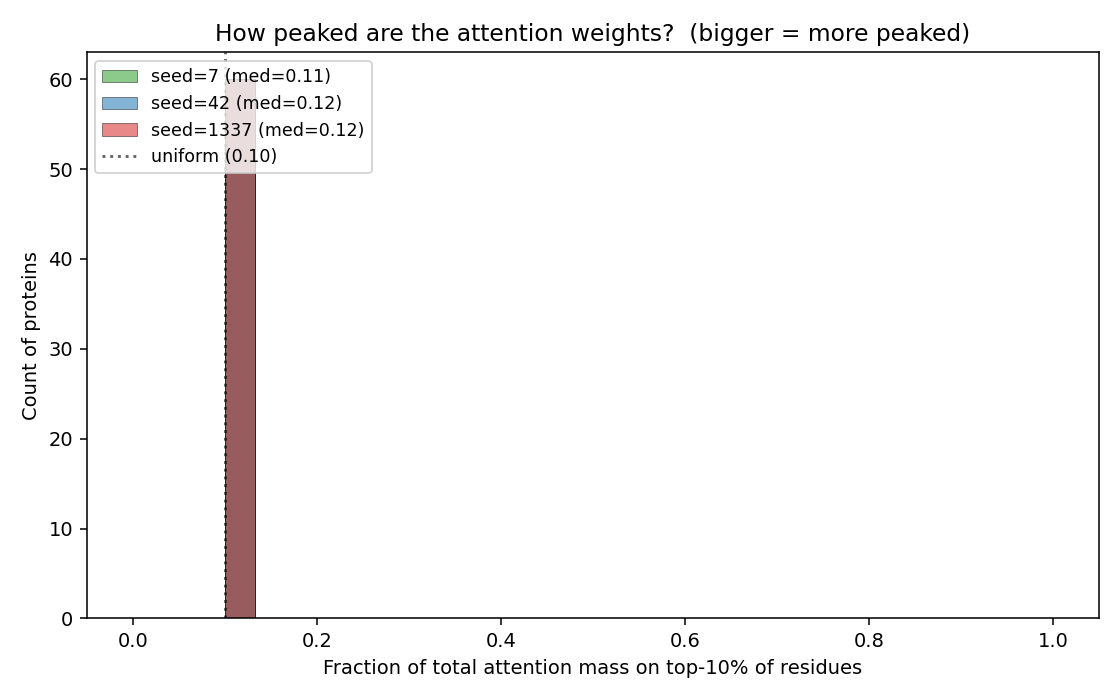
\includegraphics[width=0.8\linewidth]{fig_attn_concentration_hist.png}
  \caption{Top-$10\%$ attention-mass distribution across $60$ proteins,
  per seed. All three seeds concentrate near $0.11$--$0.12$, barely
  above the uniform expectation of $0.10$.}
  \label{fig:concentration}
\end{figure}

\paragraph{Their rank-order is reproducible across seeds.}
The same audit, on cross-seed comparisons, shows that the median
Spearman rank correlation between attention weights of independently
trained seeds is $0.86$ (random expectation $\approx 0$), and the
median top-$10\%$ residue-set Jaccard between seed pairs is $0.50$
(random expectation $\approx 0.10$); see
\Cref{fig:crossseed,fig:examples}. Three independent training runs
converge on the \emph{same} low-amplitude per-residue preference.

\begin{figure}[t]
  \centering
  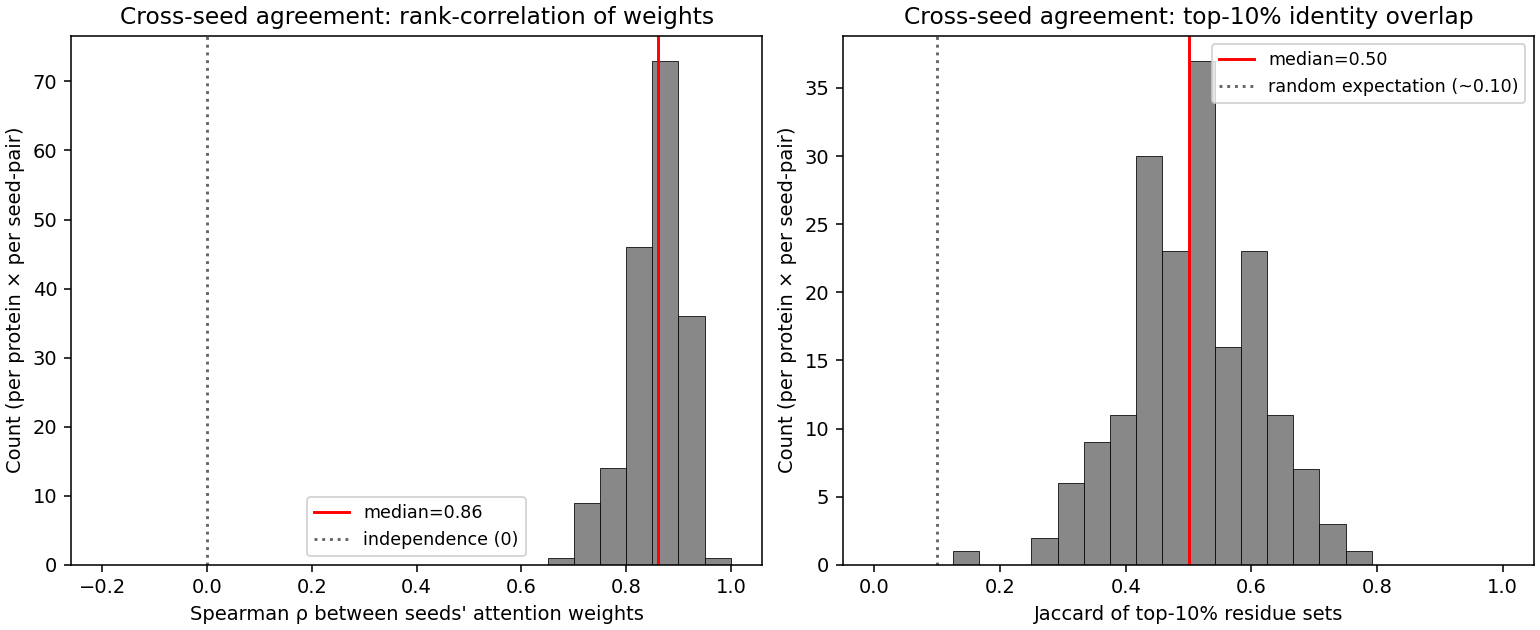
\includegraphics[width=0.95\linewidth]{fig_attn_cross_seed_agreement.png}
  \caption{Cross-seed agreement. Left: Spearman $\rho$ between
  attention weights of independently trained seeds, median $0.86$.
  Right: Jaccard of top-$10\%$ residue sets between seed pairs, median
  $0.50$ (random $\approx 0.10$).}
  \label{fig:crossseed}
\end{figure}

\begin{figure}[t]
  \centering
  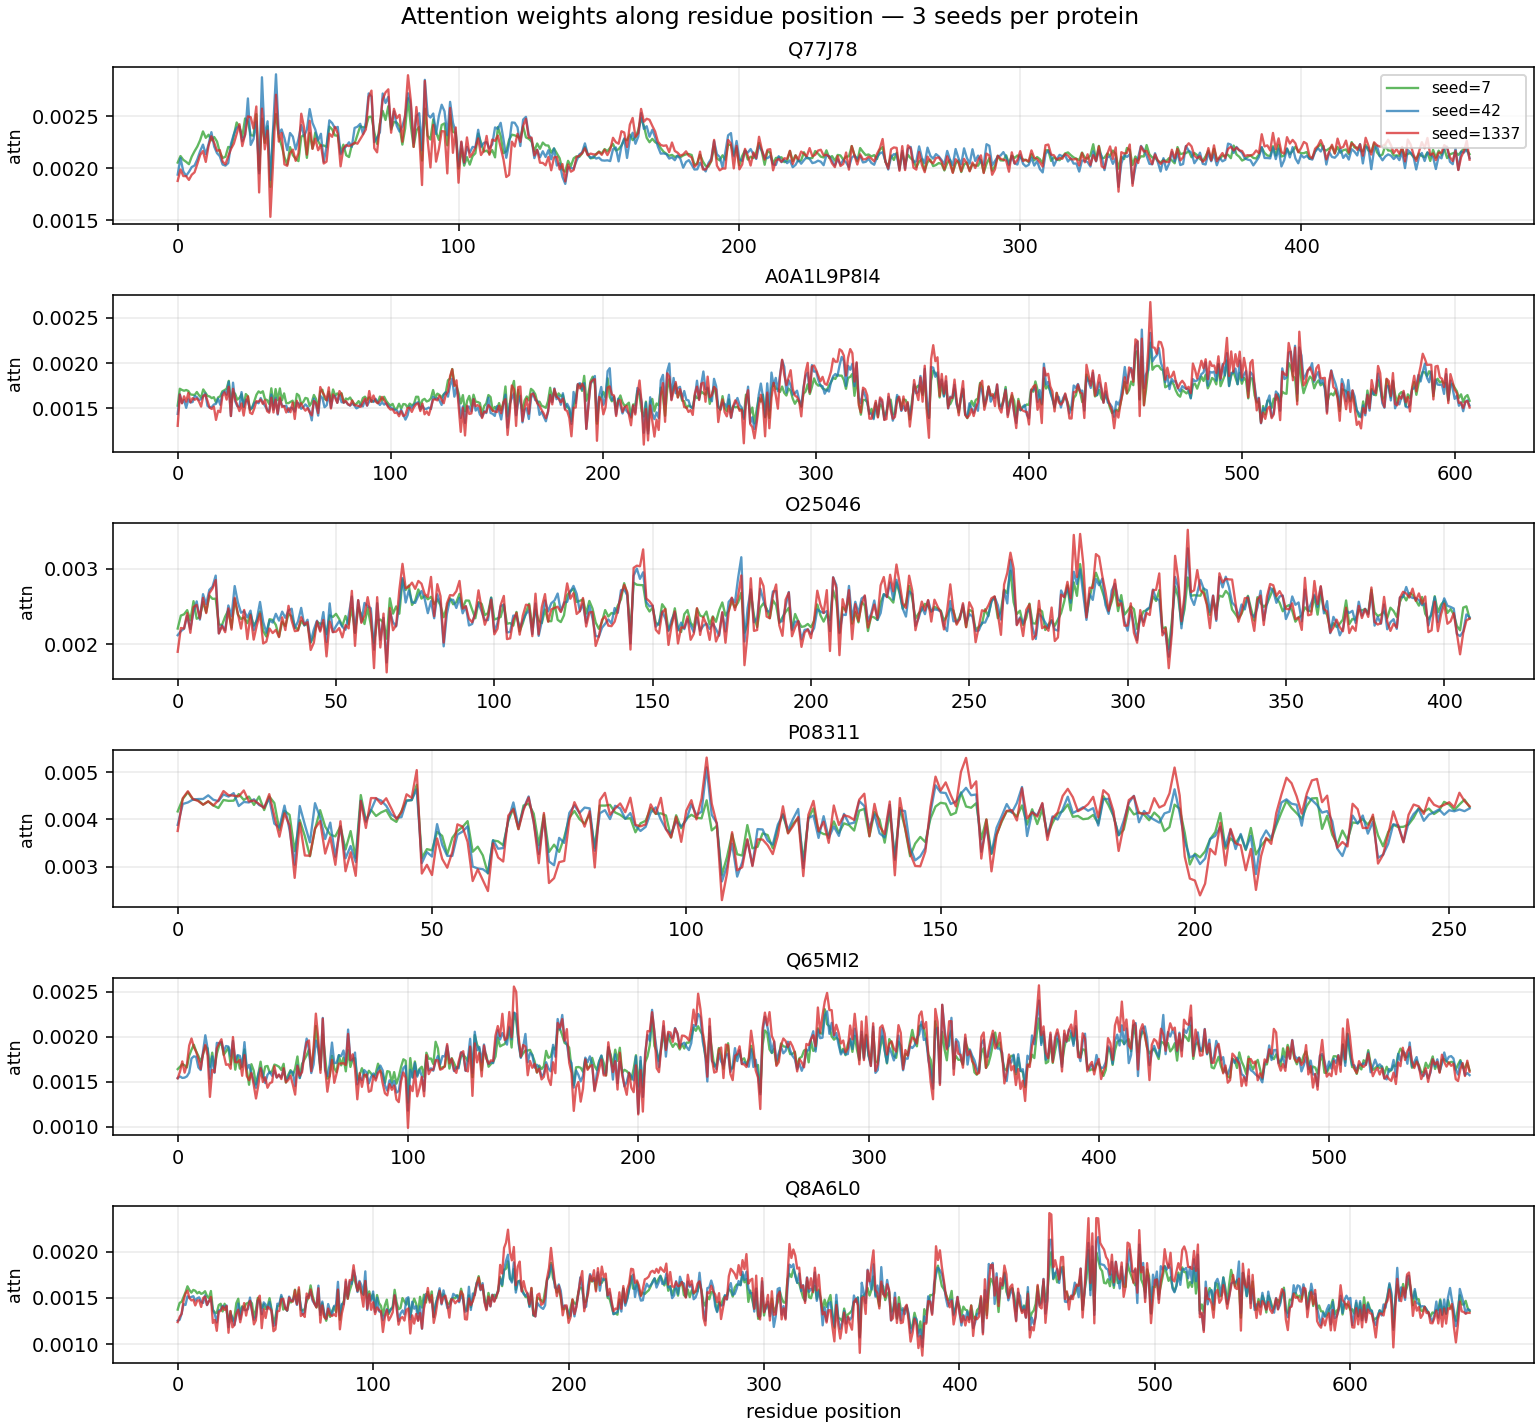
\includegraphics[width=\linewidth]{fig_attn_weight_examples.png}
  \caption{Attention weight along residue position for six example
  proteins, with three seeds overlaid per panel. Curves are jagged but
  all three seeds track each other tightly --- the y-axis range is
  small (typically $0.0015$--$0.0040$) but the shape is reproducible.}
  \label{fig:examples}
\end{figure}

\subsection{Mechanism: LayerNorm-then-pool}

The combination of near-uniform weights and reproducible rank-order
identifies \emph{LayerNorm-then-pool} as the dominant mechanism: with
near-uniform attention, the pooled representation collapses to
$\frac{1}{L}\sum_{i=1}^{L} \mathrm{LN}(\mathbf{e}_{i})$, which is
provably different from the v4 mean-pool $\frac{1}{L}\sum \mathbf{e}_{i}$.
Per-residue normalisation rescales high-norm residues (typically signal
peptides and disordered regions) so they no longer dominate the pooled
vector. The learned attention contributes the small residual.

This is itself a paper-level finding: residue-level encoding helps
\method, but the active mechanism is per-residue normalisation rather
than learned residue selection. The reproducibility of the
low-magnitude residue preference across seeds suggests that real but
subtle structural information is being picked up; quantitative pocket
overlap with M-CSA / UniProt active-site annotations is a natural
next investigation, deferred to future work.

\subsection{Implications for atom-level extension}
The originally pre-registered atom-level extension would have
identified the top-$K=8$ residues from the Stage-b attention map and
built an atom graph on those residues plus their $4$\,\AA{}
neighbourhood. The audit above blocks this mechanism empirically:
attention mass at rank-$8$ vs.\ rank-$50$ differs by $\sim 10^{-4}$,
so ``the eight most-attended residues'' is essentially a random
sample of the protein, and even consistent top-$10\%$ residue sets
overlap only $50\%$ across seeds. We therefore defer the atom-level
extension. A redesigned variant that uses AlphaFold + fpocket
structural priors instead of attention-derived pocket selection is the
only sound path forward.

% ===========================================================================
\section{Discussion}
\label{sec:discussion}

\paragraph{Generality of the diagnosis.}
The pooled-AUC vs.\ ligand-conditional-ranking gap we measure on BRENDA
is unlikely to be unique to this benchmark. Any DTI corpus where the
test protein distribution overlaps the training protein
distribution --- or where some proteins are dramatically more frequent
than others --- admits a protein-level shortcut. The null-baseline
probe is cheap (a single matrix multiply) and we recommend it as a
default sanity check before reporting pooled discrimination metrics on
new DTI datasets.

\paragraph{Cost of shortcut avoidance.}
\method explicitly trades pooled AUC for ranking quality: $0.95 \to 0.65$
in \gauc, $0.06 \to 0.33$ in \matmrr. The right benchmark for an
enzyme--substrate model is the latter --- pooled AUC certifies a
property that does not generalise across ligand identity.

\subsection{Does the recipe survive larger, enzyme-wide data?}
\label{sec:transfer}

The headline numbers in \S\ref{sec:results} are on BRENDA-200, a
hydrolase-restricted sub-corpus with $200$ unique proteins and $200$
unique ligands. To probe whether \method's anti-shortcut behaviour
persists outside that regime we re-ran the v4 default on three
BRENDA+SABIO with-decoys datasets at $50\times$ the scale (\texttt{kcat\_km}
$43$k pairs / $3.8$k proteins / $13.1$k SMILES; \texttt{km} $57$k / $9.5$k /
$14.6$k; \texttt{turnover} $42$k / $5.7$k / $13.5$k) and re-applied the
\nullprior\ probe.

\begin{table}[h]
  \centering
  \small
  \begin{tabular}{lrrr}
    \toprule
    Dataset (v4 default) & \matmrr & $\rho_{\text{row}}$ vs.\ \nullprior & Top-10 Jaccard vs.\ \nullprior \\
    \midrule
    BRENDA-200 (Phase-1 baselines)              & $0.001$--$0.06$        & n.a.                & $\mathbf{0.54\text{--}0.67}$ \\
    BRENDA-200 (\method v4)                     & $\mathbf{0.326 \pm 0.072}$ & n.a.            & $0.035 \pm 0.030$ \\
    BRENDA+SABIO \texttt{kcat\_km} (\method v4) & $0.134$                & $\mathbf{-0.008 \pm 0.062}$ & $\mathbf{0.017}$ \\
    BRENDA+SABIO \texttt{km} (\method v4)       & $0.023$                & $\mathbf{-0.134 \pm 0.026}$ & $\mathbf{0.008}$ \\
    BRENDA+SABIO \texttt{turnover} (\method v4) & $0.040$                & $\mathbf{-0.025 \pm 0.090}$ & $\mathbf{0.011}$ \\
    \bottomrule
  \end{tabular}
\end{table}

Two observations. (i) \emph{The shortcut does not return.} The mean
per-row Spearman between the v4 score matrix and \nullprior\ is at or
below zero on all three enzyme-wide datasets, and the top-10 Jaccard is
one to two orders of magnitude smaller than for the unmitigated Phase-1
baselines on BRENDA-200. The anti-shortcut property of the recipe
transfers cleanly. (ii) \emph{Absolute ranking quality drops.} Matrix
MRR falls $2$--$14\times$ from the BRENDA-200 default. Diagnostically
this is \emph{not} the Phase-1 pathology re-emerging (the model is not
just learning the per-protein training base rate); it is
signal-to-noise loss on a much harder ranking pool --- $\sim$$5$k
candidate proteins instead of $200$, and decoys drawn from a $14$k-SMILES
universe instead of $200$. The pre-registered $\texttt{hard\_pool\_size}=50$
is about $25\%$ of the BRENDA-200 train set but $0.5$--$1.3\%$ of the
BRENDA+SABIO train set, so hard-negative mining devolves toward random
sampling at this scale. Hyperparameter scaling (rather than a new
method) is the indicated intervention. We treat this as a
transferability finding for the diagnosis, not a competitive
enzyme-wide result, and defer enzyme-wide hyperparameter re-tuning to
future work.

\subsection{Practitioner recipe --- what to do for a new model or dataset}
\label{sec:recipe}

The evidence above and in \S\ref{sec:results} supports a small, ordered
recipe for any enzyme--substrate or general DTI work:

\begin{enumerate}[leftmargin=*,itemsep=2pt,topsep=2pt]
  \item \textbf{Run the \nullprior\ probe before reporting any pooled
        metric.} Score each $(L, P)$ pair on the test set using only
        the per-protein training positive rate. If the resulting
        matrix matches your model in global AUC and the top-$K$
        attractor proteins overlap heavily (Top-10 Jaccard $\ge 0.30$),
        pooled AUC has been certified by a property that does not
        depend on the ligand. Switch the primary metric to
        ligand-conditional \matmrr\ or Hit@$K$. The probe is a single
        matrix multiply and costs nothing to maintain.
  \item \textbf{Use a within-ligand margin loss as the ranking
        objective.} This is the largest single lever in our ablation:
        removing it collapses MRR by $\sim$$8\times$
        ($0.326 \to 0.041$) and the pooled AUC of the no-margin model
        rebounds to $0.95$ --- the shortcut returns. We recommend this
        loss in preference to BCE on imbalanced batches, and
        explicitly \emph{not} as an additive auxiliary: a BCE
        auxiliary at weight $0.5$ lifted \gauc\ by only $+0.03$ without
        recovering ranking quality (\S\ref{sec:gauc}).
  \item \textbf{Pair the loss with a protein-balanced sampler.} For
        each protein in the training set, draw an approximately equal
        number of positive and negative pairs per epoch. Removing this
        sampler costs $-44\%$ MRR on top of the margin loss alone,
        because heavily positive proteins re-imprint the per-protein
        prior whenever they dominate a batch.
  \item \textbf{Add online hard-negative mining, but scale
        \texttt{hard\_pool\_size} with the number of train proteins.}
        On BRENDA-200 a fixed pool of $50$ hardest non-positive
        proteins per anchor lifts MRR from $0.20$ to $0.33$ ($+62\%$).
        On BRENDA+SABIO with $3.8$--$9.5$k train proteins the same
        fixed value covers $<\!1.3\%$ of the pool and degrades to
        near-random sampling. We recommend setting
        \texttt{hard\_pool\_size} to $\sim$$10$--$25\%$ of
        $n_{\text{train\_proteins}}$ and monitoring
        \texttt{pos\_above\_neg\_max} to confirm the pool is producing
        informative negatives (it should rise into $0.95{+}$ over
        training).
  \item \textbf{Prefer a low-rank bilinear interaction head over an
        MLP-concat head.} At matched capacity ($\approx\!66$k head
        parameters) the means are similar but bilinear cuts
        seed-to-seed standard deviation by $2.2\times$ on MRR
        ($0.072$ vs.\ $0.161$), and similarly on Hit@10 and
        Gini-residual. The stability matters more than the marginal
        mean for paper-grade results.
  \item \textbf{For per-residue protein representations, normalise per
        residue before pooling.} Replacing the v4 mean-pool over
        per-residue ESM2 with a learned-query attention pool
        ($+3{,}840$ parameters, $+0.6\%$) lifted MRR $0.326 \to 0.427$.
        The attention-weight audit (\S\ref{sec:attn}) shows the
        active mechanism is per-residue LayerNorm rather than sharp
        pocket selection; a structurally-equivalent baseline that
        simply applies LayerNorm pre-pool is therefore a cheap,
        parameter-free first stop.
  \item \textbf{Do not gate model selection on pooled AUC.} Retain it
        for comparability with prior work, but on enzyme--substrate
        corpora with a skewed per-protein label distribution it
        certifies a property the ranking task should explicitly trade
        away (\S\ref{sec:gauc}). Three-seed \matmrr\ with
        seed-aware standard deviations is the metric to gate on.
  \item \textbf{Re-run the null probe on every new dataset.} A drop in
        MRR may have two distinct causes --- shortcut return or
        signal-to-noise loss at scale --- and the probe distinguishes
        them. On BRENDA+SABIO our probe rules out the first
        ($\rho \approx 0$ with \nullprior), pointing at hyperparameter
        scaling rather than an architectural problem. The opposite
        finding would have indicated the recipe needs strengthening,
        not just retuning.
\end{enumerate}

The recipe is intentionally short. The Phase-1 diagnosis identified a
single failure mode --- protein-level prior fitting --- and
\S\ref{sec:results} isolated four remedies that \emph{jointly} break it.
None of the four ingredients alone is sufficient (margin alone reaches
MRR $0.183$ without the sampler; hard-negative mining contributes
nothing without the margin); all four are needed at full strength.

\paragraph{Limitations.}
\begin{itemize}[leftmargin=*,itemsep=0pt,topsep=1pt]
  \item \textbf{\plauc{} is $n=4$.} We retain it for continuity with
        prior work but cannot draw Pass/Fail conclusions from it.
  \item \textbf{$200 \times 200$ probe matrix.} Scaling to the full
        $\sim 1.4$k-protein test pool would tighten standard errors but
        does not change the qualitative ranking.
  \item \textbf{Stage-b variance.} The MRR std grows from $0.072$ to
        $0.123$ between v4 and v5b; the mean lift is real but
        seed-to-seed spread is non-trivial and we report it
        explicitly.
  \item \textbf{No structural validation of attention weights.} The
        cross-seed Spearman of $0.86$ shows the weights agree, but we
        have not yet cross-referenced them with M-CSA / UniProt
        active-site annotations.
  \item \textbf{Out-of-distribution generalisation untested.} The
        Phase-5 cross-dataset probe (ESP, TurNuP) is scoped but not
        executed; the $+0.10$ MRR lift is therefore an in-BRENDA
        finding.
\end{itemize}

% ===========================================================================
\section{Conclusion}
\label{sec:conclusion}

We presented \method, a $627$k-parameter architecture that breaks the
protein-level shortcut on BRENDA enzyme--substrate prediction. The
core observation is methodological: pooled AUC validates the wrong
property. Against four published baselines, all of which clear pooled
AUC by exploiting the per-protein label prior, \method enforces
ligand-conditional ranking through the joint action of
protein-balanced sampling, a within-ligand margin loss, a
matched-capacity bilinear head, and online hard-negative mining. A
residue-level extension adds $+0.10$ absolute MRR and reveals that
residue-level information is best exploited via per-residue
normalisation rather than learned pocket selection. A transferability
probe on three enzyme-wide BRENDA+SABIO datasets confirms that the
recipe's anti-shortcut property survives a $50\times$ scale-up even
when absolute ranking quality does not, isolating fixed-pool
hard-negative mining as the indicated next-step intervention. We
distil the empirical findings into an eight-step practitioner recipe
for diagnosing and breaking the same shortcut on new DTI models or
datasets. We release code, configurations, three-seed manifests and
the null-prior probe so that any future enzyme--substrate model can be
audited the same way; the natural next step is to close the
enzyme-wide gap by scaling the recipe's hard-negative pool with
$n_{\text{train\_proteins}}$, alongside a cross-dataset probe on ESP
and TurNuP under distribution shift.

% ===========================================================================
\appendix
\section{Reproducibility}
\label{app:repro}

Every result in this paper is regenerable from the published
repository at a single pinned commit. The repository is split into the
parent (\texttt{rankbind/}) and a git submodule
(\texttt{reactionDataFiltering/}) that owns the dataset pipeline;
cloning with \texttt{--recurse-submodules} pins both components
together. Section~3 of the repository's \texttt{REPRODUCIBILITY.md}
lists each table and figure in this paper alongside the exact command
that emits it.

\paragraph{Hardware and environment.}
All training and evaluation runs use one NVIDIA A30 GPU on the
Leipzig HPC cluster. PyTorch~$2.8.0$ + CUDA~$12.4$ in the
\texttt{\textasciitilde/venvs/hieratombind} virtual environment.
Module load: \texttt{GCC/11.3.0 CUDA/12.4.0 Python/3.10.4-GCCcore-11.3.0}.
Mean per-seed walltime $\approx 1.5$\,h (v4) or $4$\,h (Stage-b
residue extension).

\paragraph{Data.}
BRENDA enzyme--substrate pairs with curated decoys, available at
\texttt{data/dataset\_with\_decoys.csv} (positives) +
\texttt{data/sequences/sequences.csv} (sequences) + AlphaFold
structures under \texttt{\textasciitilde/hpc/structures/}. The
protein-stratified split (seed $42$, $70/15/15$) is implemented once
in
\texttt{baselines/adapters/common.py::BRENDADataConfig.get\_protein\_split}
and reused by every model and every diagnostic.

\paragraph{Per-run provenance.}
Each training run writes a \texttt{manifest.json} under
\texttt{results/v5\_rankbind/<run\_id>/} capturing: resolved
configuration JSON (after \texttt{extends}-merging), git commit + dirty
flag, library versions, input-CSV SHA-256, split statistics, and
SHA-256 of the best-model checkpoint and $200 \times 200$ score
matrix. The manifest pins the run such that any single result in the
paper can be traced back to its exact code, configuration, and data
file content.

\paragraph{Probe code.}
The \nullprior\ probe used in \S\ref{sec:diagnosis} and
\S\ref{sec:transfer} lives at \texttt{evaluation/null\_baselines.py}
(BRENDA-200, $200 \times 200$) and
\texttt{evaluation/null\_prior\_probe\_brenda\_sabio.py} (enzyme-wide,
per-dataset). Both are runnable in under a minute on a CPU and emit
\texttt{gini\_comparison.csv} or
\texttt{null\_prior\_probe\_brenda\_sabio.csv}.

\paragraph{Multi-seed aggregation.}
The three-seed mean $\pm$ std numbers in \S\ref{sec:results} are
produced by \texttt{scripts/aggregate\_multiseed.py} walking
\texttt{results/v5\_rankbind/*\_v4*/manifest.json} and emitting
\texttt{evaluation/attractor\_results/phase2\_rankbind\_multiseed.csv}.
The same script is invoked unchanged when adding seeds.

\paragraph{Figures.}
All publication figures are regenerated by
\texttt{evaluation/phase\_d\_figures.py}; the \texttt{MATRIX\_FILES}
dictionary therein maps each model name to its
\texttt{score\_matrix\_*.npy}.

\paragraph{Hyperparameter sweep (in flight at submission).}
A Stage-1 \texttt{hard\_pool\_size} sweep over the three
BRENDA+SABIO with-decoys datasets is configured under
\texttt{v5\_rankbind/configs/sweeps/hp\_brenda\_sabio/}, with twelve
JSON configs ($4$ sweep values $\times$ $3$ datasets); submission via
\texttt{scripts/run\_v5\_brenda\_sabio\_hp\_sweep.sh}. Decision rules
for integrating sweep outcomes back into this paper are documented in
\texttt{docs/HP\_SWEEP\_INTEGRATION\_PLAN.md}.

% ---- Bibliography ---------------------------------------------------------
\bibliographystyle{plainnat}
\bibliography{references}

\end{document}
